\documentclass[]{tufte-handout}

% ams
\usepackage{amssymb,amsmath}

\usepackage{ifxetex,ifluatex}
\usepackage{fixltx2e} % provides \textsubscript
\ifnum 0\ifxetex 1\fi\ifluatex 1\fi=0 % if pdftex
  \usepackage[T1]{fontenc}
  \usepackage[utf8]{inputenc}
\else % if luatex or xelatex
  \makeatletter
  \@ifpackageloaded{fontspec}{}{\usepackage{fontspec}}
  \makeatother
  \defaultfontfeatures{Ligatures=TeX,Scale=MatchLowercase}
  \makeatletter
  \@ifpackageloaded{soul}{
     \renewcommand\allcapsspacing[1]{{\addfontfeature{LetterSpace=15}#1}}
     \renewcommand\smallcapsspacing[1]{{\addfontfeature{LetterSpace=10}#1}}
   }{}
  \makeatother

\fi

% graphix
\usepackage{graphicx}
\setkeys{Gin}{width=\linewidth,totalheight=\textheight,keepaspectratio}

% booktabs
\usepackage{booktabs}

% url
\usepackage{url}

% hyperref
\usepackage{hyperref}

% units.
\usepackage{units}


\setcounter{secnumdepth}{-1}

% citations
\usepackage{natbib}
\bibliographystyle{plainnat}


% pandoc syntax highlighting
\usepackage{color}
\usepackage{fancyvrb}
\newcommand{\VerbBar}{|}
\newcommand{\VERB}{\Verb[commandchars=\\\{\}]}
\DefineVerbatimEnvironment{Highlighting}{Verbatim}{commandchars=\\\{\}}
% Add ',fontsize=\small' for more characters per line
\newenvironment{Shaded}{}{}
\newcommand{\AlertTok}[1]{\textcolor[rgb]{1.00,0.00,0.00}{\textbf{#1}}}
\newcommand{\AnnotationTok}[1]{\textcolor[rgb]{0.38,0.63,0.69}{\textbf{\textit{#1}}}}
\newcommand{\AttributeTok}[1]{\textcolor[rgb]{0.49,0.56,0.16}{#1}}
\newcommand{\BaseNTok}[1]{\textcolor[rgb]{0.25,0.63,0.44}{#1}}
\newcommand{\BuiltInTok}[1]{#1}
\newcommand{\CharTok}[1]{\textcolor[rgb]{0.25,0.44,0.63}{#1}}
\newcommand{\CommentTok}[1]{\textcolor[rgb]{0.38,0.63,0.69}{\textit{#1}}}
\newcommand{\CommentVarTok}[1]{\textcolor[rgb]{0.38,0.63,0.69}{\textbf{\textit{#1}}}}
\newcommand{\ConstantTok}[1]{\textcolor[rgb]{0.53,0.00,0.00}{#1}}
\newcommand{\ControlFlowTok}[1]{\textcolor[rgb]{0.00,0.44,0.13}{\textbf{#1}}}
\newcommand{\DataTypeTok}[1]{\textcolor[rgb]{0.56,0.13,0.00}{#1}}
\newcommand{\DecValTok}[1]{\textcolor[rgb]{0.25,0.63,0.44}{#1}}
\newcommand{\DocumentationTok}[1]{\textcolor[rgb]{0.73,0.13,0.13}{\textit{#1}}}
\newcommand{\ErrorTok}[1]{\textcolor[rgb]{1.00,0.00,0.00}{\textbf{#1}}}
\newcommand{\ExtensionTok}[1]{#1}
\newcommand{\FloatTok}[1]{\textcolor[rgb]{0.25,0.63,0.44}{#1}}
\newcommand{\FunctionTok}[1]{\textcolor[rgb]{0.02,0.16,0.49}{#1}}
\newcommand{\ImportTok}[1]{#1}
\newcommand{\InformationTok}[1]{\textcolor[rgb]{0.38,0.63,0.69}{\textbf{\textit{#1}}}}
\newcommand{\KeywordTok}[1]{\textcolor[rgb]{0.00,0.44,0.13}{\textbf{#1}}}
\newcommand{\NormalTok}[1]{#1}
\newcommand{\OperatorTok}[1]{\textcolor[rgb]{0.40,0.40,0.40}{#1}}
\newcommand{\OtherTok}[1]{\textcolor[rgb]{0.00,0.44,0.13}{#1}}
\newcommand{\PreprocessorTok}[1]{\textcolor[rgb]{0.74,0.48,0.00}{#1}}
\newcommand{\RegionMarkerTok}[1]{#1}
\newcommand{\SpecialCharTok}[1]{\textcolor[rgb]{0.25,0.44,0.63}{#1}}
\newcommand{\SpecialStringTok}[1]{\textcolor[rgb]{0.73,0.40,0.53}{#1}}
\newcommand{\StringTok}[1]{\textcolor[rgb]{0.25,0.44,0.63}{#1}}
\newcommand{\VariableTok}[1]{\textcolor[rgb]{0.10,0.09,0.49}{#1}}
\newcommand{\VerbatimStringTok}[1]{\textcolor[rgb]{0.25,0.44,0.63}{#1}}
\newcommand{\WarningTok}[1]{\textcolor[rgb]{0.38,0.63,0.69}{\textbf{\textit{#1}}}}

% longtable

% multiplecol
\usepackage{multicol}

% strikeout
\usepackage[normalem]{ulem}

% morefloats
\usepackage{morefloats}


% tightlist macro required by pandoc >= 1.14
\providecommand{\tightlist}{%
  \setlength{\itemsep}{0pt}\setlength{\parskip}{0pt}}

% title / author / date
\title[様々な分布を確認する]{様々な分布を確認する}
\author{Sampo Suzuki, CC 4.0 BY-NC-SA}
\date{2021-06-29}

% --- 参考資料 ----------------------------------------------------------------
% http://ctan.math.illinois.edu/language/japanese/zxjafont/zxjafont.pdf
% https://github.com/Gedevan-Aleksizde/Japan.R2019/blob/master/latex/preamble.tex
% https://teastat.blogspot.com/2019/01/bookdown.html

% --- Packages ----------------------------------------------------------------
% 日本語とtufte, kableExtraを使うために必要なTeXパッケージ指定
% \usepackage[pdfbox,tombo]{gentombow}    % トンボを設定する場合は有効にする
\usepackage{ifthen}                     % 条件分岐用 \ifthenelse{条件}{T}{F}
\usepackage{booktabs}                   % ここからkableExtra用パッケージ
\usepackage{longtable}                  % 
\usepackage{array}                      % 
\usepackage{multirow}                   % 
\usepackage{wrapfig}                    % 
\usepackage{float}                      % 
\usepackage{colortbl}                   % 
\usepackage{pdflscape}                  % 
\usepackage{tabu}                       % 
\usepackage{threeparttable}             % 
\usepackage{threeparttablex}            % 
\usepackage[normalem]{ulem}             % 
\usepackage{inputenc}                   % 
\usepackage{makecell}                   % 
\usepackage{xcolor}                     % ここまでkableExtra用
\usepackage{amsmath}                    % 
\usepackage{fontawesome5}               % fontawesomeを使うために必要
\usepackage{subfig}                     % 複数の図を並べる際に必要(古い?)
% \usepackage{subcaption}                 % 同上(新しい?)
\usepackage{zxjatype}                   % 日本語処理に必要
% \usepackage{xeCJK}                      % zxjatypeを読み込むと一緒に読み込まれる
\usepackage[noto]{zxjafont}             % Linux環境用
% \usepackage[haranoaji]{zxjafont}        % Windows環境用
% \usepackage[hiragino-pro]{zxjafont}     % macOS環境用(おそらく、駄目ならNotoで)
\usepackage{pxrubrica}                  % ルビ用
\usepackage{hyperref}                   % ハイパーリンク用必要?
% 以下のパッケージについては下記サイトを参照方
% http://www.yamamo10.jp/yamamoto/comp/latex/make_doc/box/box.php
% \usepackage{ascmac}                     % 別行で文書を囲む場合
% \usepackage{fancybox}                   % 行中で文書を囲む場合 fancybx ではない
% \usepackage{fancyhdr}                   % ヘッダー用

% https://ja.wikibooks.org/wiki/TeX/LaTeX%E5%85%A5%E9%96%80
% https://teastat.blogspot.com/2019/01/bookdown.html

\begin{document}

\maketitle




\hypertarget{ux6a19ux672cux6a19ux6e96ux504fux5deeux306fux3069ux306eux3088ux3046ux306aux5206ux5e03ux3092ux53d6ux308bux306eux304b}{%
\section{標本標準偏差はどのような分布を取るのか?}\label{ux6a19ux672cux6a19ux6e96ux504fux5deeux306fux3069ux306eux3088ux3046ux306aux5206ux5e03ux3092ux53d6ux308bux306eux304b}}

 『統計解析の話』\citep{ToukeiKaisekinoHanashi}では母集団のばらつき(母標準偏差
\(\sigma\))を推定するために母集団からサンプリングした標本の標準偏差(\(s\))の分布を用いようと説明されています\footnote{3.
  名探偵ものがたり ばらつきを区間推定するには P56〜}。そこで、標本標準偏差(\(s\))をの分布をテキストにあるように以下の手順で求めてみます。

\begin{enumerate}
\def\labelenumi{\arabic{enumi}.}
\tightlist
\item
  標本数を\(n = 2\)とする
\item
  母集団\footnote{建前上は未知の母集団}から上記の標本を取り出す
\item
  標本から標本標準偏差(\(s\))を計算して記録する
\item
  上記を任意の回数\footnote{本資料では1万回}繰り返す
\item
  記録した標本標準偏差(\(s\))のヒストグラムをプロットする
\end{enumerate}

\begin{Shaded}
\begin{Highlighting}[numbers=left,,]
\NormalTok{n }\OtherTok{\textless{}{-}} \DecValTok{2}
\NormalTok{df }\OtherTok{\textless{}{-}} \FunctionTok{data.frame}\NormalTok{()}
\ControlFlowTok{for}\NormalTok{ (i }\ControlFlowTok{in} \FunctionTok{c}\NormalTok{(}\DecValTok{1}\SpecialCharTok{:}\DecValTok{10000}\NormalTok{)) \{}
\NormalTok{  xs }\OtherTok{\textless{}{-}} \FunctionTok{rnorm}\NormalTok{(n)}
\NormalTok{  dftmp }\OtherTok{\textless{}{-}} \FunctionTok{data.frame}\NormalTok{(}\AttributeTok{no =}\NormalTok{ i, }\AttributeTok{s =} \FunctionTok{sqrt}\NormalTok{(}\FunctionTok{sum}\NormalTok{((xs }\SpecialCharTok{{-}} \FunctionTok{mean}\NormalTok{(xs))}\SpecialCharTok{\^{}}\DecValTok{2}\NormalTok{) }\SpecialCharTok{/}\NormalTok{ n))}
\NormalTok{  df }\OtherTok{\textless{}{-}}\NormalTok{ dplyr}\SpecialCharTok{::}\FunctionTok{bind\_rows}\NormalTok{(df, dftmp)}
\NormalTok{\}}
\end{Highlighting}
\end{Shaded}

\begin{figure}

{\centering 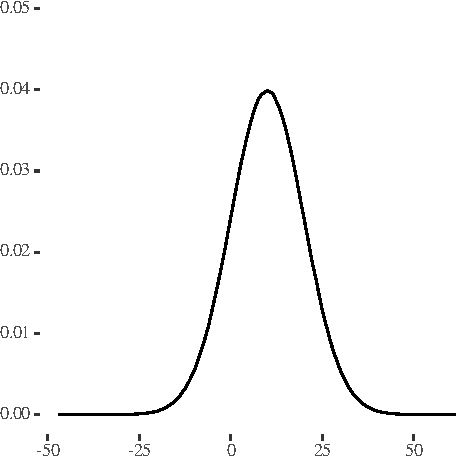
\includegraphics[width=0.8\linewidth]{StandardDivision_files/figure-latex/unnamed-chunk-2-1} 

}

\caption[標本標準偏差の分布]{標本標準偏差の分布}\label{fig:unnamed-chunk-2}
\end{figure}

このように大きく右に歪んだ分布になることがわかります\footnote{次ページと比較しやすいように横軸をそろえてあります。縦軸は異なるので注意してください。}。

\newpage

次に同じ手順で母集団の標準偏差(\(\sigma\))が異なると標本標準偏差(\(s\))の分布がどのようになるかを確認します。

\begin{figure*}

{\centering \subfloat[母標準偏差=3\label{fig:unnamed-chunk-3-1}]{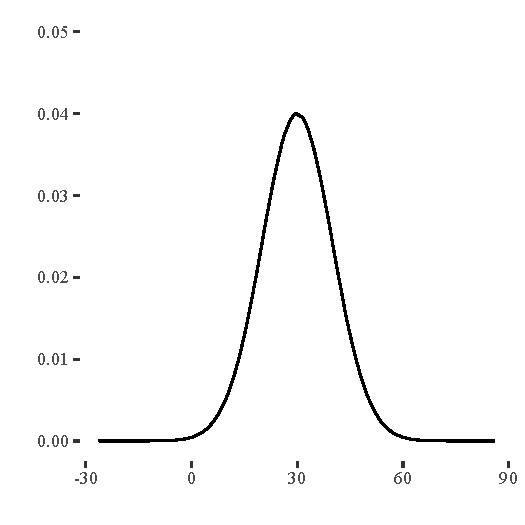
\includegraphics[width=0.45\linewidth]{StandardDivision_files/figure-latex/unnamed-chunk-3-1} }\subfloat[母標準偏差=5\label{fig:unnamed-chunk-3-2}]{\includegraphics[width=0.45\linewidth]{StandardDivision_files/figure-latex/unnamed-chunk-3-2} }

}

\end{figure*}

母標準偏差(\(\sigma\))が大きくなると右側にながらかになることがわかります。

 

では、母標準偏差を変えずに標本数(サンプリング数)を変えた場合、どのような分布になるでしょうか?

\begin{figure*}

{\centering \subfloat[標本数=3\label{fig:unnamed-chunk-4-1}]{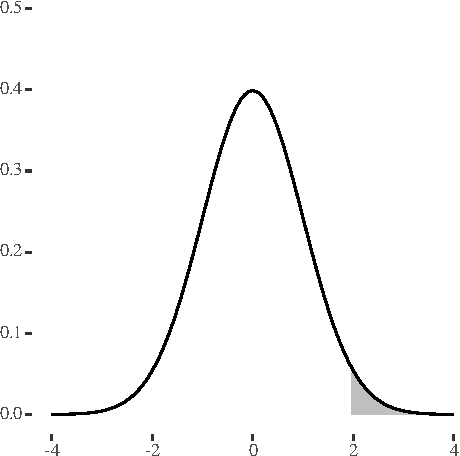
\includegraphics[width=0.45\linewidth]{StandardDivision_files/figure-latex/unnamed-chunk-4-1} }\subfloat[標本数=10\label{fig:unnamed-chunk-4-2}]{\includegraphics[width=0.45\linewidth]{StandardDivision_files/figure-latex/unnamed-chunk-4-2} }

}

\end{figure*}

標本数が大きくなると母標準偏差(\(\sigma\))を中心とした正規分布に近づいていくことがわかります。

\newpage

\hypertarget{ux504fux5deeux5e73ux65b9ux548cux306eux5206ux5e03}{%
\section{偏差平方和の分布}\label{ux504fux5deeux5e73ux65b9ux548cux306eux5206ux5e03}}

 テキスト\citep{ToukeiKaisekinoHanashi}では計算を簡単にするために標本標準偏差ではなく偏差平方和\footnote{3.
  名探偵ものがたり ばらつきを区間推定するには P57〜}の分布を求めるようにしています。では、偏差平方和\footnote{\(S = \sum_{i = 1}^{n}{(x_i - \bar{x})^2}\)}の分布がどのようになるかプロットしてみます。偏差平方和は数式を見て分かるように標本標準偏差\footnote{\(s = \sqrt{\frac{\sum_{i = 1}^{n}{(x_i - \bar{x})^2}}{n}}\)}と比例関係にありますので、分布形状も比例するはずです。

\begin{Shaded}
\begin{Highlighting}[numbers=left,,]
\NormalTok{n }\OtherTok{\textless{}{-}} \DecValTok{2}
\NormalTok{df }\OtherTok{\textless{}{-}} \FunctionTok{data.frame}\NormalTok{()}
\ControlFlowTok{for}\NormalTok{ (i }\ControlFlowTok{in} \FunctionTok{c}\NormalTok{(}\DecValTok{1}\SpecialCharTok{:}\DecValTok{10000}\NormalTok{)) \{}
\NormalTok{  xs }\OtherTok{\textless{}{-}} \FunctionTok{rnorm}\NormalTok{(n)}
\NormalTok{  dftmp }\OtherTok{\textless{}{-}} \FunctionTok{data.frame}\NormalTok{(}\AttributeTok{no =}\NormalTok{ i, }\AttributeTok{S =} \FunctionTok{sum}\NormalTok{((xs }\SpecialCharTok{{-}} \FunctionTok{mean}\NormalTok{(xs))}\SpecialCharTok{\^{}}\DecValTok{2}\NormalTok{))}
\NormalTok{  df }\OtherTok{\textless{}{-}}\NormalTok{ dplyr}\SpecialCharTok{::}\FunctionTok{bind\_rows}\NormalTok{(df, dftmp)}
\NormalTok{\}}
\end{Highlighting}
\end{Shaded}

\begin{figure}

{\centering 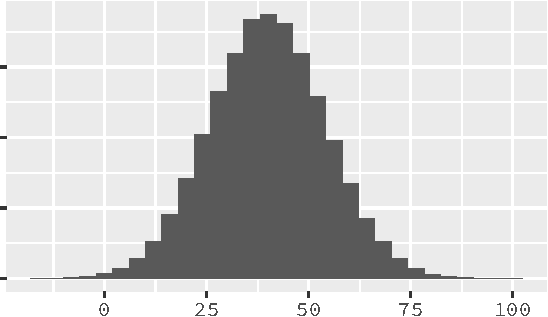
\includegraphics[width=0.8\linewidth]{StandardDivision_files/figure-latex/unnamed-chunk-6-1} 

}

\caption[偏差平方和の分布]{偏差平方和の分布}\label{fig:unnamed-chunk-6}
\end{figure}

また、テキスト\footnote{3. 名探偵ものがたり
  ばらつきを区間推「定するにはP58}にあるように母標準偏差(\(\sigma\))で分布が変わるかどうかを確認します。

\begin{figure*}

{\centering \subfloat[母標準偏差=3\label{fig:unnamed-chunk-7-1}]{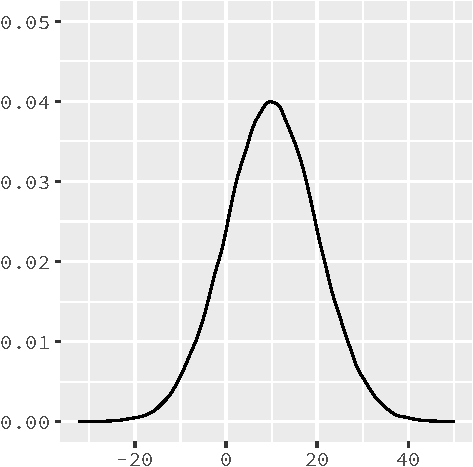
\includegraphics[width=0.45\linewidth]{StandardDivision_files/figure-latex/unnamed-chunk-7-1} }\subfloat[母標準偏差=5\label{fig:unnamed-chunk-7-2}]{\includegraphics[width=0.45\linewidth]{StandardDivision_files/figure-latex/unnamed-chunk-7-2} }

}

\end{figure*}

\newpage

\hypertarget{chi2ux5206ux5e03}{%
\section{\texorpdfstring{\(\chi^2\)分布}{\textbackslash chi\^{}2分布}}\label{chi2ux5206ux5e03}}

 \(\chi^2\)分布\footnote{\(\chi^2 = \frac{S}{\sigma^2} = \frac{\sum_{i = 1}^{n}{(x_i - \bar{x})^2}}{\sigma^2}\)}は標本数(自由度)により分布が変わりますが、母集団の標準偏差(\(\sigma\))には左右されないという特徴があります。

\begin{Shaded}
\begin{Highlighting}[numbers=left,,]
\NormalTok{n }\OtherTok{\textless{}{-}} \DecValTok{2}
\NormalTok{sd }\OtherTok{\textless{}{-}} \DecValTok{1}
\NormalTok{df }\OtherTok{\textless{}{-}} \FunctionTok{data.frame}\NormalTok{()}
\ControlFlowTok{for}\NormalTok{ (i }\ControlFlowTok{in} \FunctionTok{c}\NormalTok{(}\DecValTok{1}\SpecialCharTok{:}\DecValTok{10000}\NormalTok{)) \{}
\NormalTok{  xs }\OtherTok{\textless{}{-}} \FunctionTok{rnorm}\NormalTok{(n, }\AttributeTok{sd =}\NormalTok{ sd)}
\NormalTok{  dftmp }\OtherTok{\textless{}{-}} \FunctionTok{data.frame}\NormalTok{(}\AttributeTok{no =}\NormalTok{ i, }\AttributeTok{S =} \FunctionTok{sum}\NormalTok{((xs }\SpecialCharTok{{-}} \FunctionTok{mean}\NormalTok{(xs))}\SpecialCharTok{\^{}}\DecValTok{2}\NormalTok{), }\AttributeTok{var =}\NormalTok{ sd }\SpecialCharTok{\^{}} \DecValTok{2}\NormalTok{)}
\NormalTok{  df }\OtherTok{\textless{}{-}}\NormalTok{ dplyr}\SpecialCharTok{::}\FunctionTok{bind\_rows}\NormalTok{(df, dftmp)}
\NormalTok{\}}
\end{Highlighting}
\end{Shaded}

\begin{figure}

{\centering 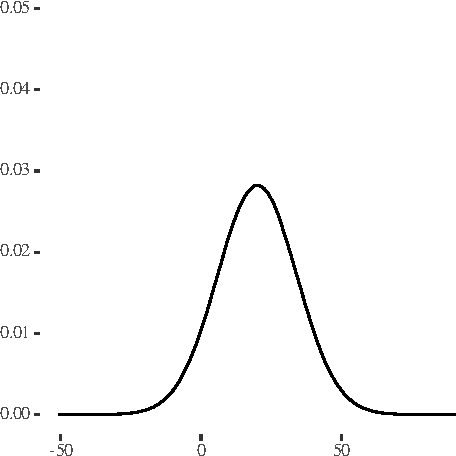
\includegraphics[width=0.8\linewidth]{StandardDivision_files/figure-latex/unnamed-chunk-9-1} 

}

\caption[自由度=1の$\chi^2$分布]{自由度=1の$\chi^2$分布}\label{fig:unnamed-chunk-9}
\end{figure}

 \\
自由度を変えた場合。

\begin{figure}

{\centering \subfloat[自由度=3\label{fig:unnamed-chunk-10-1}]{\includegraphics[width=0.4\linewidth]{StandardDivision_files/figure-latex/unnamed-chunk-10-1} }\subfloat[自由度=5\label{fig:unnamed-chunk-10-2}]{\includegraphics[width=0.4\linewidth]{StandardDivision_files/figure-latex/unnamed-chunk-10-2} }

}

\caption[自由度が異なる$\chi^2$分布]{自由度が異なる$\chi^2$分布}\label{fig:unnamed-chunk-10}
\end{figure}

\newpage

母集団の標準偏差(\(\sigma\))を変えた場合。

\begin{figure}

{\centering \subfloat[母標準偏差=3\label{fig:unnamed-chunk-11-1}]{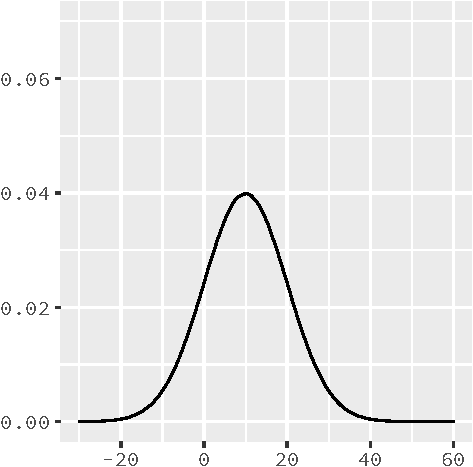
\includegraphics[width=0.4\linewidth]{StandardDivision_files/figure-latex/unnamed-chunk-11-1} }\subfloat[母標準偏差=10\label{fig:unnamed-chunk-11-2}]{\includegraphics[width=0.4\linewidth]{StandardDivision_files/figure-latex/unnamed-chunk-11-2} }

}

\caption[自由度=3の$\chi^2$分布]{自由度=3の$\chi^2$分布}\label{fig:unnamed-chunk-11}
\end{figure}

\bibliography{bib/references.bib}



\end{document}
